\documentclass[a4paper, 11pt, oneside, polutonikogreek, french]{article}
\usepackage{lmodern}
\usepackage[T1]{fontenc}

% Load encoding definitions (after font package)

\usepackage{textalpha}

\usepackage{listings}
\lstset{basicstyle=\ttfamily}

% Babel package:
\usepackage[french]{babel}

% With XeTeX$\$LuaTeX, load fontspec after babel to use Unicode
% fonts for Latin script and LGR for Greek:
\ifdefined\luatexversion \usepackage{fontspec}\fi
\ifdefined\XeTeXrevision \usepackage{fontspec}\fi

% "Lipsiakos" italic font `cbleipzig`:
\newcommand*{\lishape}{\fontencoding{LGR}\fontfamily{cmr}%
		       \fontshape{li}\selectfont}
\DeclareTextFontCommand{\textli}{\lishape}

% Load encoding definitions (after font package)
\usepackage{eso-pic,graphicx}
\usepackage[top=50mm, bottom=58mm, outer=33mm, inner=33mm]{geometry}
\setlength{\columnsep}{90pt}
\definecolor{customColor}{RGB}{230, 231, 233}

\usepackage{booktabs}
\setlength{\emergencystretch}{15pt}
\usepackage{fancyhdr}
\usepackage{microtype}
\usepackage{setspace}
\onehalfspacing
\makeatletter % change only the display of \thepage, but not \thepage itself:
\patchcmd{\ps@plain}{\thepage}{\bfseries\color{customColor}{\thepage}}{}{}
\makeatother

\color{customColor}
\begin{document}
\bfseries
\renewcommand\thefootnote{\bfseries{\arabic{footnote}}}
\let\oldfootnote\footnote
    \renewcommand{\footnote}[1]{\oldfootnote{\bfseries#1}}
    
\AddToShipoutPictureBG{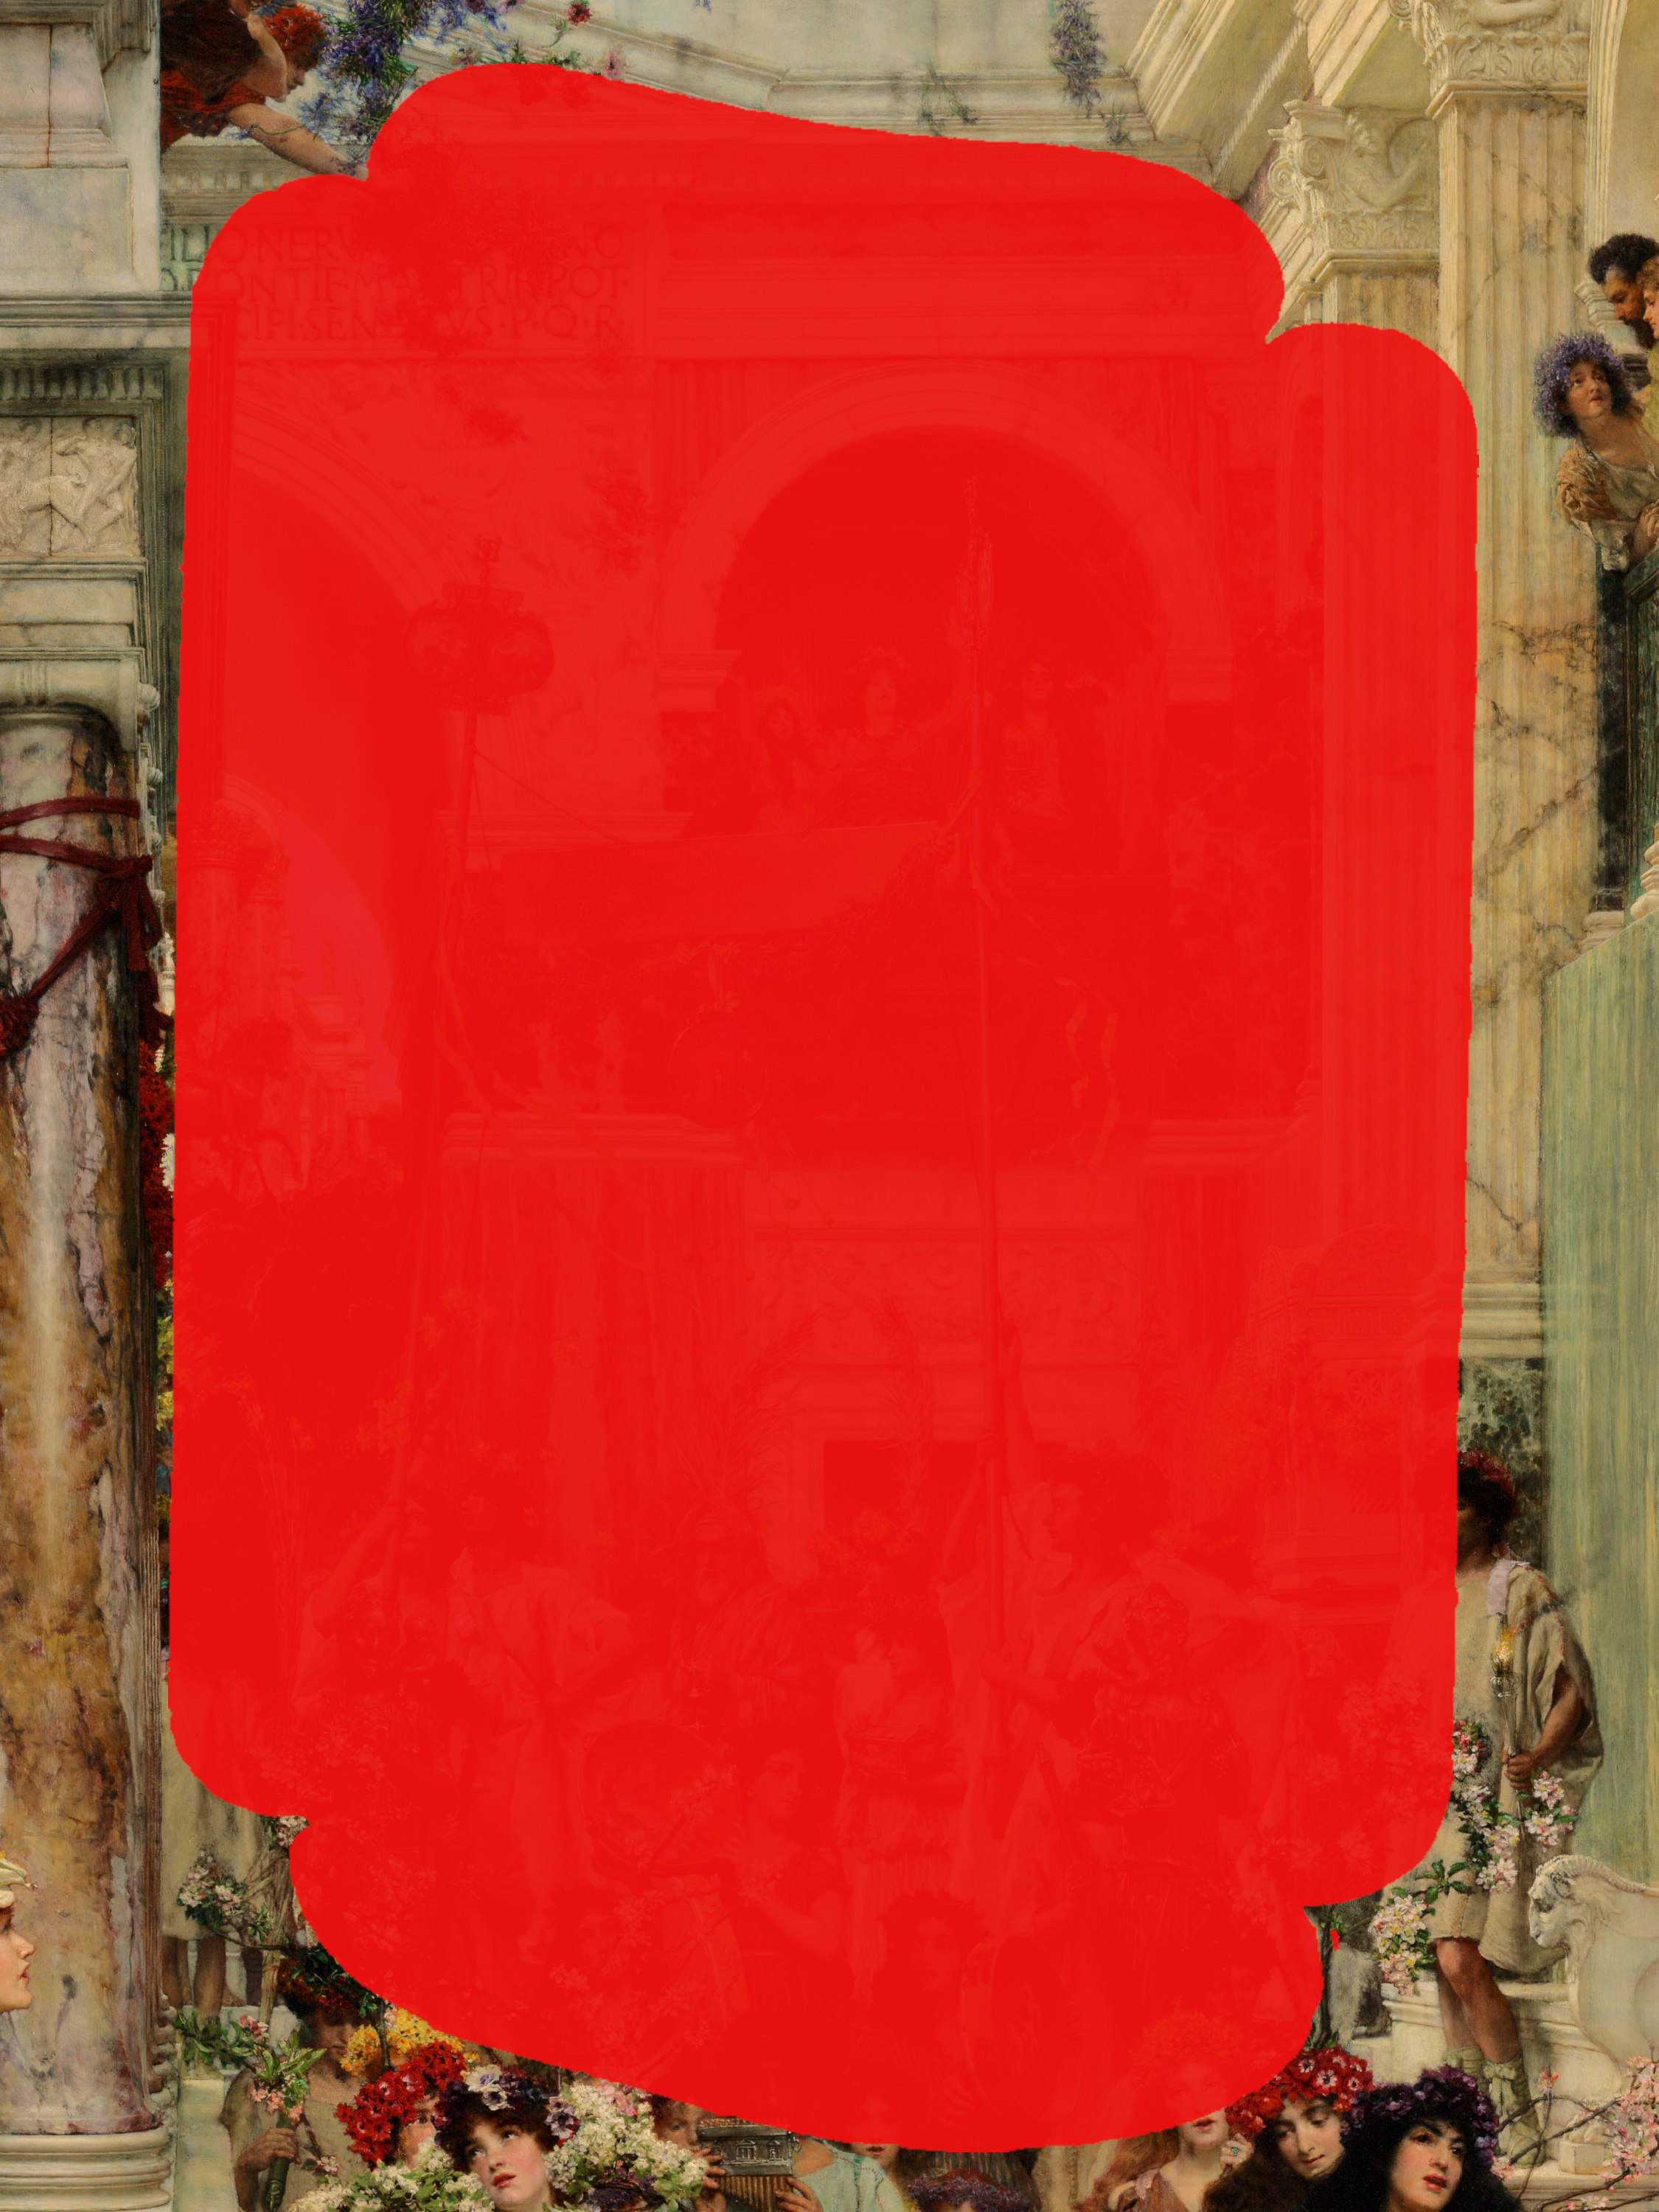
\includegraphics[width=\paperwidth,height=\paperheight]{roman3.jpeg}}
\begin{titlepage} % Suppresses headers and footers on the title page
	\centering % Centre everything on the title page
	%\scshape % Use small caps for all text on the title page

	%------------------------------------------------
	%	Title
	%------------------------------------------------
	
	\rule{\textwidth}{1.6pt}\vspace*{-\baselineskip}\vspace*{2pt} % Thick horizontal rule
	\rule{\textwidth}{0.4pt} % Thin horizontal rule
	
	\vspace{1\baselineskip} % Whitespace above the title
	
	{\scshape\Huge Dissertation sur la Pierre de la Mère des Dieux.}
	
	\vspace{1\baselineskip} % Whitespace above the title

	\rule{\textwidth}{0.4pt}\vspace*{-\baselineskip}\vspace{3.2pt} % Thin horizontal rule
	\rule{\textwidth}{1.6pt} % Thick horizontal rule
	
	\vspace{1\baselineskip} % Whitespace after the title block
	
	%------------------------------------------------
	%	Subtitle
	%------------------------------------------------
	
	{\scshape \Large Par M. Falconet} % Subtitle or further description
	
	\vspace*{1\baselineskip} % Whitespace under the subtitle
	
        {\scshape\scriptsize } % Subtitle or further description
    
	%------------------------------------------------
	%	Editor(s)
	%------------------------------------------------
        \vspace*{\fill}

	\vspace{1\baselineskip}

	{\small\scshape Paris 21 Avril 1750.}
	
	{\small\scshape{De L'Imprimerie Royal}}
	
	\vspace{0.5\baselineskip} % Whitespace after the title block

        \scshape Internet Archive Online Edition  % Publication year
	
	{\scshape\small Utilisation non commerciale --- Partage dans les mêmes conditions 4.0 International} % Publisher
\end{titlepage}
\setlength{\parskip}{1mm plus1mm minus1mm}
\clearpage
\large
\paragraph{}
En 1722 je lus une Dissertation sur les Bétyles, où, à l'occasion de ces pierres, je fis mention de plusieurs autres d'une forme singulière, parmi lesquelles je me contentai d'indiquer la grandeur et la configuration de la pierre de la mère des Dieux ; j'entends cette pierre regardée comme le simulacre de la Déesse que les Romains firent venir de Pessinonte, ville de Galatie,\footnote{Cicéron, que je cite plus bas, dit, \emph{sacra ex Phrygia ascita}. Strabon, \emph{liv. 12}, dit qu'une partie de la Galatie est comprise sous le nom de Phrygie.} sur ce que les livres Sibyllins consultés avoient déclaré que l'arrivée de cette pierre à Rome opèrerait l'expulsion d'Annibal et des Carthaginois hors de l'Italie.

Comme le fond de ce fait historique appartient à la mythologie, M. l'abbé Banier, très-versé dans cette partie de la Littérature, crut devoir me faire quelques objections sur la petitesse que j'attribuais à cette pierre, et lut même ensuite à l'Académie quelques remarques, où il tachait d'établir un sentiment contraire au mien. M. de Boze donna l'extrait de ces remarques dans l'histoire de l'Académie\footnote{Tome 5.} ; peu de temps après je lus un Mémoire, où à mon tour je tâchai de confirmer, par de nouvelles preuves, ce que je n'avois dit qu'en passant, dans ma Dissertation sur les Bétyles : je ne donnai point alors ce Mémoire à nos registres, comptant d'y ajouter de nouveaux éclaircissements concernant la mère des Dieux ; qu'il me soit permis de présenter aujourd'hui ce même Mémoire comme neuf, du moins en meilleur état qu'il n'était d'abord. Il ne reste au plus que sept où huit Académiciens du temps où j'en fis la lecture (c'était en 1722), je souhaite que mes nouveaux Confrères, qui n'en ont aucune connaissance, ne le jugent pas tout-à-fait indigne de leur curiosité.

La translation de la pierre de la mère des Dieux de Pessinonte à Rome, l'an de Rome 548, est un fait historique dont plusieurs auteurs ont fait mention ; Ovide, Tite-Live, Silius Italicus, Appien, Hérodien, parmi un grand nombre d'autres,\footnote{Denys d'Halicarnasse n'est point de ce nombre, ainsi que l'a cru M. l'abbé Banier, \emph{Hist. de l'Acad.} tome 5, page 242. Ce que nous avons des antiquités Romaines de cet historien, finit à l'an de Rome 312 ; s'il avait eu dessein de faire mention de ce fait, il l'aurait sans doute rapporté dans l'endroit où il parle de l'introduction des mystères de Cybèle à Rome, \emph{l. 2.}} sont ceux qui en parlent avec plus de détail : mais la narration de la plupart n'a point pour objet de nous représenter ni la grandeur ni la figure de la pierre de la mère des Dieux. Pour ce qui regarde la grandeur, Tite-Live est celui qui nous donne le plus précisément à entendre que la pierre ne devait être ni d'une grandeur ni d'un poids fort considérable, lorsqu'il dit que Scipion Nasica, l'ayant reçue de dessus le vaisseau qui l'avait apportée, la remit entre les mains des dames Romaines, qui successivement la portèrent jusqu'au temple de la victoire : \emph{In terram elatam tradidit (Scipio Nasica) ferendam Matronis... eæ per manus, succedentes alæ aliis... in ædem Victoriæ pertulere.} On trouve dans Silius Italicus à peu près là même chose,\footnote{Liv. 17, v. 16.} \emph{femineæ tum deinde manus subiere}, et nous rapporterons plus bas un passage d'Arnobe, où il est dit que la pierre de la mère des Dieux était si petite, que son poids ne se faisait pas sentir à la main ; ainsi quand les dames Romaines se la donnèrent successivement à porter, comme dit Tite-Live, ce n'était pas pour se soulager d'un poids trop pesant, comme l'a cru M. l'abbé Banier, c'était pour partager entre elles l'honneur de porter la mère des Dieux.\footnote{Orat. de Harus. respons. S. 13.} Cicéron\footnote{Cicéron dit, Orat. de Haruspic. responsis, \emph{sacra ista ex Phrygiâ ascita Romæ collocaverunt, quæ is (Scipio) accepit... femina autem Q. Claudia, etc.} Je ne rapporte le passage que pour faire remarquer que Cicéron, par le mot \emph{sacra}, désigne la pierre de la Déesse ; Ovide se sert du même mot, \emph{Fastor. l. 4, vers. 340, Dominam sacraque lavit aquis}, et Diodore, \emph{extract. ex lib. 34}, dit en grec τὰ ἱερά. Au reste cet historien est le seul qui, au même endroit, appelle \emph{Valeria} celle que tous les autres nomment \emph{Claudia}.} ne fait mention que de Q. Claudia pour cette honorable fonction, Tite-Live la nomme parmi les autres Dames, et quelques auteurs font de Claudia une vestale ; j'indique dans une note la cause de leur erreur.\footnote{Hérodien, \emph{liv. 1, c. 2}, fait de \emph{Claudia} une vestale, ἥπς τῆς Ἐστίας, il la confond avec \emph{Claudia} vestale qui monta hardiment sur le char de triomphe de son frère. \emph{V. Suetone Tiber. c. 2. Cartari imagin. pag. 179}, a suivi avec d'autres l'erreur d'Hérodien. Des miracles de cette espèce, opérés par quelques vestales, ont sans doute donné lieu à faire croire que Claudia était vestale aussi. Denys d'Halicarnasse, \emph{liv. 2}, parle des vestales \emph{Æmilia et Tuccia}, toutes deux soupçonnées, qui se justifièrent, l'une en rallumant le feu sacré éteint, par un morceau de sa robe de lin qu'elle y jeta, l'autre en portant de l'eau dans un crible. Plusieurs auteurs ont parlé de cette dernière, \emph{Valère-Maxime, liv. 8, chap. 1, S 5, Pline, liv. 28, c. 2, Florus Epitom. liv. 20, Tertul. Apologet. c. 22, S. August. de civitate Dei, l. 10, c. 16}. Je remarquerai à cette occasion une faute de Pline ; il met le fait de Tuccia à l'an de Rome 609, Merula, \emph{p. 77, commentar. ad Ennium}, le met en 519 sur un passage de l'épitome de Florus : le passage est décisif, quel qu’effort que fasse le P. Hardouin pour défendre Pline.} Ovide ajoute le miracle\footnote{Fastor. l. 4.} qu'à l'arrivée du vaisseau à l'embouchure du Tibre opéra cette matrone, dont jusqu'alors la chasteté avait été suspecte. Claudia ayant imploré le secours de la mère des Dieux pour sa justification, attacha sa ceinture au vaisseau et le dégagea sans effort de la vase du Tibre, d'où aucune force n'avait pu le tirer. Silius Italicus, Pline, Suétone, Hérodien et beaucoup d'autres\footnote{\emph{Cingulo duxit navem}, dit S. Jerôme, l. 1, \emph{contra Jovinianum}.} ont répété cette dernière histoire, mais elle est étrangère à notre sujet ; il nous suffit que cette pierre, que des modernes ont cru avoir besoin d'une paire de bœufs pour être remuée, ainsi que nous verrons bientôt, se trouve ici portée à la main par une seule femme.

Ovide cependant rapporte que la Déesse,\footnote{Fastor. l. 4.} c'est-à-dire sa pierre, entra à Rome par la porte Capène sur un char traîné par des génisses : mais je crains qu'Ovide n'ait confondu la cérémonie de la lavation de la mère des Dieux, avec celle de la première entrée de la Déesse à Rome sous la forme d'une pierre. Je ne sais même, si l'on doit croire, avec ce Poète, que la Déesse, en arrivant, fut d'abord lavée dans le fleuve Almon : Tite-Live dit qu'elle fut portée immédiatement au temple de la Victoire. La cérémonie de la lavation ne fut sans doute célébrée que dans la suite. Les Pretres, pour engager plus fortement le peuple dans la superstition, introduisirent bientôt la coutume de baigner la statue de la Déesse, et ne firent en cela qu'imiter la pratique religieuse des Grecs. Ezéchiel Spanheim a donné là-dessus une note\footnote{\emph{In lavacrum Palladis}.} curieuse dans ses observations sur Callimaque. J'ajoute à cette note que les nations septentrionales pratiquaient dans leur Religion une semblable cérémonie pour la même divinité. Tacite dit que les Germains voisins\footnote{\emph{De moribus Germanorum}, c. 40.} de la mer Baltique, qui adoraient la déesse de la Terre sous le nom de \emph{Herthus} où \emph{Herta}, la baignaient dans un lac le jour de sa fête\footnote{Voy. Erd. terra Wachter. Gloss. Germanic.} : \emph{Numen ipsum secreto lacu abluitur : servi ministrant quos statim idem lacus haurit}.

Revenons à Ovide : quand il serait plus digne de foi que Cicéron et Tite-Live, on ne peut point conclure de la voiture du char, pour la grosseur de la pierre, ce qui se conclut, pour sa petitesse, de la facilité que les femmes avoient à la porter ; un gros fardeau ne peut se porter à la main, et un très-petit peut être mis sur un très-grand char, surtout si une cérémonie n'en devient que plus auguste. C'est sur un pareil char que dans la suite, pour faire honneur à la Déesse, on voiturait en grande pompe la pierre, ou plutôt la statue où la pierre était enchâssée, comme nous verrons bientôt, pour la laver dans le fleuve Almon tous les ans, au jour nommé \emph{lavatio} dans le calendrier Romain.\footnote{Sur la fin de mars, \emph{6 calend. aprilis. Vibius Sequester de fluminibus}, au mot \emph{Almon, Romæ ubi mater Deûm 6 calend. aprilis lavatur.} Pareille fête fut placée sur la fin de février dans le même calendrier sous le nom de \emph{Lotio} pour la déesse Pallas. \emph{Voy. Ezéch. Spanheim ci-dessus.}} J'ajouterai ce qui, je crois, a échappé à nos mythologistes modernes. Il y eut un cas particulier où le fleuve Almon ne paraissant pas suffisant pour calmer la Déesse qui avait donné des marques de sa colère, il fallut la porter à la mer. Dion rapporte ce fait à l'an de Rome 716.\footnote{50. 48 de son histoire.} On avait porté la Déesse à la mer pour pareille cause plus de soixante ans auparavant, l'an de Rome 651.\footnote{Voyez l'histoire de Battacès ou Batabacès, prêtre de Cybèle, dans Plutarque \emph{in Mario} et dans les extraits de Photius \emph{ex lib. 36 Diodori.}}

Vincent Cartari, dans son livre des images des Dieux,\footnote{\emph{Seconda editione delle imagini de Gli Dei.} Padua, 1626, in-4°.} a sans doute pris de la cérémonie dont nous venons de parler, l'idée qu'il a eue de a figure de la pierre de la mère des Dieux, et la représentation qu'il en a donnée\footnote{50. 48 de son histoire. Pag. 1792.} : \emph{Il simulacro}, dit-il, \emph{di questa Dea portato all' hora della Frigia fa un grand pietra nigra, etc.} et il la représente comme un grand cône tronqué, élevé sur un char trainé par des bœufs. Pignoria, savant Antiquaire, se contente dans ses notes d'alléguer Hérodien, Arnobe et d'autres auteurs,\footnote{\emph{Ibid.}, p. 483-4.} sans marquer le moindre soupçon sur l'erreur de Cartari : mais ce qui doit étonner beaucoup davantage, c'est que Réinésius, Critique exact, d'une profonde érudition, ait non seulement adopté l'imagination de Cartari, mais encore ait cru l'autoriser en nous donnant, pour l'idole de la mère des Dieux,\footnote{Variar. lection. lib. 3, c. 17, p. 637.} une masse de pierre tirée du mont \emph{Agdus} ; voici l'histoire qui a donné lieu à la confusion des idées de ce savant homme.\footnote{Adversus Gentes. l. 5.} Arnobe voulant expliquer l'origine des mystères de la mère des Dieux, dit que, selon Timothée,\footnote{Alb. Fabricius, bibl. Grecq. ni aucun autre auteur ne m'apprend quel est ce Timothée, entre tant d'autres qui ont porté le même nom ; serait-ce le Milésien dont Grotius rapporte un vers grec sur la pudeur. \emph{Excerpta ex Tragæd}, 1626, in-4°. pag. 456.} théologien Payen de réputation, il y avait en Phrygie un rocher d'une vaste grandeur, appelé \emph{Agdus} ; que ce fut de-là que Deucalion et Pyrrha prirent les pierres dont ils réparèrent le genre humain ; que la mère des Dieux elle-même fut formée d'une de ces pierres ; que sur ce même rocher ensuite Jupiter ayant voulu forcer Cybèle, mais inutilement, le rocher Agdus reçut le principe de la fécondation, d'où il conçut et mit au jour un enfant monstrueux appelé \emph{Agdestis},\footnote{On trouve la mère des Dieux nommée elle-même Αγγιδιστις Αγδιστις (terminaison plus convenable au sexe féminin) dans Strabon et dans Hésychius. \emph{Voy les notes sur ces deux auteurs des éditions données dans ce siècle-ci, ce qui est confirmé par une inscription}, pag. 97, Miscellan. erudit. Antiquit. à J. Sponio, 1685, \emph{fol.}} dont les aventures se trouvent ensuite mêlées avec celles d'Attis. Je ne puis m'empêcher de dire en passant qu'une bonne partie de cette narration fabuleuse pourrait bien ne devoir son origine qu'à une mauvaise traduction qu'aura faite Arnobe du texte grec de ce Timothée. J'en conçois une forte présomption sur les vers latins qu'il nous rapporte au sujet de Cérès : on y voit une version obscure et infidèle des vers grecs du prétendu Orphée, que nous a conservés Clément Alexandrin. Au reste, cette histoire d'\emph{Agdus} et d'\emph{Agdestis} est rapportée assez différemment dans Pausanias\footnote{Achaïcorum, c. 17.} : on en trouve aussi quelques vestiges qui la défigurent encore davantage dans le Plutarque \emph{de fluminibus}, à l'article d'\emph{Araxes} ; Mithras y est nommé au lieu de Jupiter, et Diorphus au lieu d'Agdestis. Les premiers Pères de l'Eglise\footnote{S. Justin \emph{advers. Tryphonem}, Jul. Firmic. Matern. \emph{de errore profanar. religion.} S. Jerôme, \emph{l. 1., advers. Jovinianum}, et d'après eux Commodien, \emph{instruction 13}.} ont encore changé les personnages de cette fable ; c'est Mithras même qui, selon eux, est né de la pierre Θεὸς σκ πέτρας, \emph{invictus de petra Deus}. Ce serait abuser de son temps que de chercher à concilier tant démontreuses absurdités : il est bien plus important de remarquer, en finissant cet article, que cette pierre du rocher \emph{Agdus}, transformée réellement, selon Timothée, en Cybèle vivante et animée, ne peut avoir rien de commun avec la pierre de la mère des Dieux qui demeura toujours pierre.

Réinésius s'est donc trompé. On n'en saurait douter. C'est ainsi qu'on trouve en défaut, avec Réinésius, les Scaligers, les Saumaises, \emph{etc.} quand on veut approfondir en particulier certains points qu'ils n'ont traités qu'incidemment dans de grands ouvrages. Ces Savants qui passent pour être du premier ordre, parce qu'ils embrassent toutes les parties de la Littérature, regardent comme un temps dérobé à l'acquisition de nouvelles connaissances, celui qu'ils emploieraient à vérifier les faits et à citer exactement les auteurs. Il serait même souvent à souhaiter qu'ils s'en tinssent à cette négligence, et qu'ils n'allassent pas jusqu'à altérer les textes par l'extrême envie qu'ils ont de les accommoder à leurs opinions singulières.

Pour confirmer ce que nous avons dit sur le peu de volume de la pierre de la mère des Dieux, examinons sa figure et l'usage qui fut fait de cette pierre, nous verrons que l'un et l'autre conviennent parfaitement à la petitesse que nous lui avons assignée. Il est singulier qu'aucun des auteurs que nous avons cités, à l'exception d'un seul, ne spécifie la figure de la pierre de la Déesse : c'est la mère des Dieux, disent simplement Ovide, Tite-Live, Sil. Italicus, \emph{etc.} dans Cicéron encore plus vaguement, \emph{sacra ista ex Phrygia ascita Romæ, etc.}\footnote{Voyez ci-dessus la note sur Cicéron et Diodore.} : Diodore dit de même, τὰ ἱερά ; Tite-Live l'appelle \emph{sacrum lapidem} ; dans Claudien\footnote{De raptu Proserpinæ, l. 1, vers. 202.} c'est \emph{relligiosa silex}, dans Hérodien, ἄγαλμα ; avant lui Strabon avait dit ἀφίδρυμα, Appien, βρέτας ; et d'après eux Amm. Marcellin,\footnote{50. 1, c. 2.} \emph{simulacrum}. Remarquons en passant,\footnote{50. 12.} qu'Appien, Hérodien et Amm. Marcellin sont les seuls qui disent que le simulacre était tombé du Ciel : Hérodien ajoute qu'on en ignorait la matière aussi-bien que l'ouvrier.

Il semblerait que le mot de \emph{simulacre} indiquerait quelque ressemblance à la chose représentée ; mais on se tromperait : tout ce qui faisait l'objet de l'Idolâtrie dans ces premiers temps où elle devança la sculpture, quelque figure qu'il eût, portait le nom de \emph{simulacre}, comme si ç'avoient été des statues. Les Celtes adoraient Jupiter\footnote{Maxim. Tyr. Dissert. 38.} sous la forme d'un chêne : une souche, un tronc coupé à Thespies, et une planche\footnote{Clem. Alexandr. \emph{Prot. c. 4.}, σανὶς est mal rendu, \emph{stipes} par le traducteur, \emph{pluteus} mieux dans Arnobe, \emph{l. 6} ; le fait est pris de Callimaque. \emph{Voy, fragment 105} et \emph{la note de Bentley.}} à Samos furent les premières idoles de Junon\footnote{Maxim. Tyr. Dissert. 38. et Clem. Alexandr. Proc. c. 4.} ; Minerve, \emph{inter Deos ergatas}, Ἀθήνη ἐργάνη, et Apollon,\footnote{Pausan. liv. 8, c. 32.} ἀγυιεὺς, étaient représentés par des pierres carrées ; Latone à Délos,\footnote{Athenée, l. 14, c. 1.} Diane à Icare étaient des morceaux de bois informes ; la statue d'Apollon\footnote{Clem. Alexandr. Stromat. \emph{liv. 1, chap. 24}, voyez aussi Pausanias Corinth. \emph{liv. 2, chap. 9 et 29}, et Harpocration au mot Ἀγυιᾶς.} à Delphes était une colonne\footnote{Clem. Alexand. Protrept. c. 4.} ; et sept colonnes dans la Laconie représentaient les sept planètes : Castor et Pollux à Sparte étaient figurés par deux poutres parallèles,\footnote{Pausan. Lacon. l. 3, c. 20.} traversées près de leurs extrémités par deux autres. Selon Plutarque\footnote{\emph{Plut. initio libri} πρὶ Φιλαδελφίας. M. Huet traduit δὁκανα par \emph{trabalia, Animadvers. in Manil. pag. 82}, le P. Calmet \emph{in Genes. c. 28}, lit mal δονάκια.} qui décrit cette figure, Δόκανα était leur nom ; les Gémeaux sont ainsi désignés par les Astronomes, et cette figure a passé dans nos almanachs : une pierre pyramidale était la Vénus de Paphos\footnote{Tacite, \emph{historiar. l. 2, c. 2 et Maxim. Tyr. Dissert. 38. Vide Cuper. in Lactant. de mortib. persecutor. pag. 158, édit. de Bauldri.} Sous la même forme pyramidale étaient adorés le Soleil à Èmèse, \emph{Hérodien, liv. 5, chap. 3}, Jupiter Milichius à Sicyone, \emph{Pausan}. \emph{Corinthiac. lib. 2, cap. 9}, et Apollon Carinus à Mégare, \emph{Paus. Atticor. l. 1, c. 44.}} (on la voit sur les médailles) ; de simples pierres,\footnote{\emph{Tertullian. apologet. c. 16, Ceres Pharia quæ... rudi palo et informi ligno prostat}.} sans aucune figure particulière, étaient les idoles de l'Amour\footnote{\emph{Pausan. Bœoticor. lib. 9, c. 24 et 27}, il parle aussi, \emph{Achaïcor. l. 7, c. 22}, de trente pierres carrées adorées comme autant de Dieux à Pharès.} à Thespies, et d'Hercule à Hyète : une pierre carrée\footnote{\emph{Pocock specimen historiæ Arabum, pag. 114, 121, 122, et Bochart Phaleg. l. 2, c. 19}.} servait également et d'idole et d'autel aux Arabes ; ainsi que chez les Dymatiens\footnote{Χρῶνται Δουμαθηνοὶ ὡς ξοάνῳ, \emph{etc. Porphyr. de abstinentia carn. l. 2., c. 56, v.} Δοὐμαθα \emph{dans Steph. Doumata Igiandal}, ainsr nommé aujourd'hui, lieu de l'Arabie déserte, qui sépare la Syrie de l'ancienne Chaldée. \emph{Voy. Laroque, description de l'Araie.}} de la même nation, un autel tenait lieu de statue. Je pousserais cette énumération bien plus loin ; mais il me suffit de remarquer que les auteurs qui rapportent tous ces faits, emploient des mots de la même valeur que celui de \emph{simulacre}, pour exprimer ces objets représentatifs d'une divinité avec laquelle ils n'avoient aucune ressemblance. Il semble que les premiers hommes regardaient comme impossible\footnote{\emph{Clem. Alexandr.} τὸ ἀνει κόνιστον τοῦ θεοῦ. \emph{Stromat. l. 1, c. 24.}} de représenter des Dieux qui étaient invisibles.\footnote{Ἀόρατοι, ἀμόρφωτοι, ἀτύπωτοι. \emph{v. Ezech. Spanh. in lavacr. Pallad. Pag. 595.}} C'est peut-être par cette raison que Clément Alexandrin dit qu'on se servait de colonnes, non comme d'une image, mais simplement comme d'un signe.\footnote{Ce qu'il dit des colonnes, Justin le dit des lances, \emph{ab origine rerum pro Diis immortalibus hastas coluere}, lib. 43, cap. 3, \emph{vide Cuper. Apotheos. Homer. p. 22.}} Nous n'avons donc rien à conclure sur la figure de la pierre de la mère des Dieux, des mots ἄγαλμα, ἀφίδρυμα, βρέτας, ξόανον, \emph{simulacrum}, dont on s'est servi pour la désigner.

Arnobe, de tous les auteurs anciens qui sont parvenus jusqu'à nous, est le premier qui ait décrit cette pierre d'une manière à nous donner l'idée de sa figure, aussi-bien que de sa grandeur : la voici telle qu'on la voyait de son temps et qu'il l'a vue lui-même.\footnote{\emph{Arnob. advers. Gentes}, lib. 7, pag. 253, édit. Batav. in-4°.} \emph{Allatum ex Phrygia nihil quidem aliud... nisi lapis quidam non magnus, ferri manu hominis sine ulla impressione qui posset, coloris furvi atque atri, angellis prominentibus inæqualis, et quem omnes hodie ipso illo videmus in signo oris loco positum, indolatum et asperum, et simulacro faciem minus expressam simulatione præbentem}. On voit dans cette description une petite pierre qui peut être portée à la main sans faire sentir son poids, \emph{ferri manu sine ulla impressione qui posset} : cette pierre est noire, raboteuse, irrégulière par ses angles ; mais au milieu de cette irrégularité, elle montre une apparence de bouche ; et cette ressemblance, quoiqu'imparfaite, donne l'idée d'enchâsser la pierre dans le visage d'une statue pour y tenir lieu de bouche : j'ajoute et par-là cette statue devient celle de la divinité que l'on croit cachée sous la figure de la pierre. Tel est le sens que présente très-clairement, et sans équivoque, le texte d'Arnobe. Prudence, s'il était nécessaire, confirmerait cette interprétation dans deux vers qui eux-mêmes ont besoin du passage d'Arnobe pour être entendus.

\emph{Lapis nigellus evehendus essedo,}  

\emph{Muliebris oris clausus argento sedet.*}\footnote{Hymn. 10, παρὶ στεφάνων, vers. 156-7.}

Les interprètes\footnote{Iso Magister, moine de saint Gal du 9e. siècle, explique \emph{lapis nigellus} par \emph{gagates}, c'est, à ce que l'on croit, le pissasphalte ou le bitume pétrifié ; Carol. Néapolis dit sans balancer, \emph{magnis vere creditus Anaptyxis, in Ovid. Fastor. l. 4, v. 340.}} de ce Poète ne disent rien de raison nable sur ce passage : le savant Cuper\footnote{\emph{In Lactant. de mortib. persecutor.} p. 157 de l'édit de Bauldri.} lui-même paraît fort embarrassé de ces mots \emph{muliebris oris}, parce qu'aucun d'eux n'a recours au passage d'Arnobe. Prudence nous apprend de plus qu'on avait enchâssé la pierre dans de l'argent, sans doute pour la rendre plus remarquable : il indique aussi la cérémonie où la Déesse était portée sur un char, par ces mots \emph{evehendus essedo.}

C'est donc sur une pareille configuration dépeinte avec tant de précision, que, dans ma Dissertation sur les Bétyles, j'osai affirmer ce que j'affirme encore à présent, que nous avions sous nos yeux aujourd'hui la pierre de la mère des Dieux ; sur quoi j'avançai que cette pierre était de l'espèce de ces petites pierres noires dont les bords sont anguleux et inégaux, au milieu desquels se voit un sillon bien marqué, et que les Naturalistes de ces derniers siècles ont nommées \emph{hystérolithes}, par rapport à une ressemblance qui n'est guère éloignée de celle d'une bouche. Je conjecturai de plus que ce fut cette ressemblance regardée comme un grand mystère, qui donna occasion au culte de fa pierre, et qu'il fut aisé à la superstition de se persuader que, sous une semblable figure, se présentait elle-même aux mortels une Déesse qui, selon les Poètes, était la mère des Dieux et des hommes ; et félon les Philosophes, était a Nature même, source unique de tout ce qui paraît dans l'Univers.

C'est dans ce même sens qu'il faut prendre le mot \emph{Hystera} que St. Irénée\footnote{\emph{Lib. 1, contra hæreses, c. 35 de Caianis (qui et Caini, Cainiani) : jam autem et collegi eorum conscriptiones, in quibus dissolvere opera hysteræ adhortantur ; hysteram autem fabricatorem cœli et terræ vocant} : ce premier livre n'est qu'en latin depuis le chap. 22 jusqu'au 31 inclusivement. On croit cette traduction latine, pleine de grécismes, faite du temps de la vulgate. \emph{Voy. Billius observat. l. 1, c. 33.} S. Irénée, \emph{c. 17}, en grec du même livre, avait déjà dit que les Marcosiens, disciples de Marcus le Valentinien, enseignaient que le fabricateur avait opéré la création, sans le savoir lui-même, par le ministère de la mère, τὴς κτίσιν ὑπὸ τοῦ Δημιουργοῦ, ὡς ἀγνοονῦτος ἀυταρ καταστκευάσθαι δζα τῆς Μηρὸς λέγουσι. Par ce passage on voit manifestement que l'\emph{hystera} du chapitre 31 est ici appelé \emph{mater}. De tout cela on peut conjecture avec grande raison que ces hérétiques, tels qu'on nous les donne, les plus grands visionnaires qu'il y ait jamais eus, avoient emprunté de la mythologie l'idée que l'on y avait de la mère des Dieux, ce qui me paraît plus vraisemblable que l'explication du mot \emph{hystera}, donnée par D. Massuet, \emph{in Irenæum Dissert. 1, S 157}. Ajoutons encore, que comme chez les Païens, Cybèle avait plusieurs noms, Γῆ, Θέμις, Ἴσις, \emph{etc.} de même chez ces hérétiques le mère était appelée Ὀγδιὰς, Σοφία, Γῆ, où l'on voit le mot Γῆ de part et d'autre ; sur quoi il y a encore à remarquer, à l'occasion de cette Ὀγδιὰς, ce que dit Nicomachus Gerasenus, ἡ Ὀκτὰς, πρῶτος ἐνεργεία κύβος, était regardée par les Pythagoriciens comme Rhéa, Cybèle, \emph{etc.} \emph{voy. Photius, Cod. 187}, et selon eux sans doute le nom de Κυβέβη venait de Κύβος.} emploie comme le nom qu'on avait donné au fabricateur du Ciel et de la Terre, dont les ouvrages avoient été attaqués par certains hérétiques. St. Epiphane\footnote{\emph{Panarii sive adversus Hæreses, l. 1, c. 3}, où après avoir parle de l'évangile de Judas (c'est l'Iscariote, qui, selon ces hérétiques, était de leur secte) il ajoute : και ἄλλα πνὰ συγνράμματα ὡσαύτως πλάττονταικατα τῆς ὑστέρας ἣν ὑστέραν τειν ποιητὴν τοῦ restitués παήσος τούσου τοῦ κύσους οὐρανου της και τῆς γῆς καλοῦσι, passage qui doit être regardé comme le texte grec original de S. Irénée, dont nous avons rapporté la traduction latine dans la note précédente. S. Épiphane, au commencement de cet article, avait mis les Sodomites avec Caïn, Ésaii, Coré, comme tous de la même secte, et avait remarqué que, selon ces hérétiques, Ève ayant eu affaire avec deux puissances, eut Caïn de la plus forte et Abel de la plus faible, \emph{etc.}} copie St. Irénée à l'article des Caïniens, qu'il dit s'être déclarés les ennemis de ce fabricateur (ποιητὴς), nommé \emph{Hystera}. Le P. Pétau n'a pas jugé à propos de s'engager dans aucune explication de ce passage : tout obscur qu'il paraît, on voit cependant que la conjecture de ceux\footnote{\emph{Theodor. Hasæus de Saxonum idolo Ostera, Bibl. Bremens. t. 15, p. 496-7}, où de plus il se trompe quand il dit \emph{hysteram} à \emph{Caianis fuisse cultam}, c'est précisément le contraire. Au reste, Rhenferdius, qu'il cite comme étant de son sentiment, peut avoir raison en ce qu'il croit qu'il n'y a point eu d'hérétiques Caïnites, et que par ce mot on ne doit entendre que les impies opposés aux descendons d'Abel et de Seth.} qui voudraient substituer \emph{Astarte à Hystera}, ne saurait être admise. Saint Epiphane, au même endroit, oppose manifestement Caïn, E'sau, Coré et les Sodomites, comme tous d'une même secte, aux partisans du fabricateur \emph{Hystera}.

Rien ne convenait donc mieux à une divinité regardée comme la Nature même, que le titre de mère des Dieux ; aussi le voit-on communément sur les médailles et dans les inscriptions, quelquefois \emph{magna mater},\footnote{Au dessous de la statue de la Déesse. \emph{Boissard, l. 6, pl. 37}.} \emph{mater magna},\footnote{\emph{Inscrip. Gruter. p. 1065, 8}, et \emph{M. Gudii}, p. 20-1.} sans addition : bien plus \emph{Ma},\footnote{\emph{Stephan. de urbibus voca} Μάσταυρα.} chez les Lydiens, était le nom de \emph{Rhea}, comme Mère par excellence ; sur quoi il est assez curieux d'observer que tous les mots employés pour dire mère\footnote{M. de la Condamine, dans sa relation de la rivière des Amazones, \emph{p. 56}, observe que les mots \emph{Abba} ou \emph{Papa} et \emph{Mama} sont communs à un grand nombre de nations d'Amérique, quoique leur langage soit d'ailleurs très-différent.} chez presque tous les peuples du monde entier, ont la lettre \emph{m} pour radicale, comme une labiale que les enfans prononcent dès qu'ils commencent à balbutier.

Je trouve dans un monument rapporté par Pausanias, une épithète très-convenable à la qualité de mère. Cet\footnote{\emph{50. 5, c. 13}, ἐν τῇ κορυφῇ τοῦ ὄρους (Σιπὑζου) τῆς Πλαστήνς Μηρὸς τὸ ἱερόν.} auteur dit que, sur le mont Sipyle, il y avait un temple de la mère Plastène : je rendrais volontiers ce mot par le \emph{fabricator} de St. Iréné, ou le ποιητὴς de St Epiphane. Kuhnius, dernier éditeur de Pausanias, ne fait aucune remarque sur ce mot oublié par tous les lexicographes : rien de plus naturel que sa formation, πλαστήνη de πλαστὴς, comme πθήνη de πτθός, \emph{etc.}

A l'occasion du mont Sipyle,\footnote{Tantalis, Sipyle et trois autres villes bâties successivement au même lieu, toutes cinq abîmées par des tremblemens de terre. \emph{Voy. Pline, liv. 5, chap. 29}. Magnésie, qui prit ensuite leur place, fut très-fort endommagée par les tremblemens suivans. Le mont Sipyle et Magnésie sont près de Smyrne vers l'embouchure de l'Hermus ; Cellarius, \emph{geograph. antiq.} se méprend très-fort quand il les place presque à la source de ce fleuve dans sa carte de l'Asie mineure.} nom que portait aussi la ville voisine, je me contenterai de dire que c'était sur cette montagne où le même Pausanias dit ailleurs,\footnote{50. 3. c. 22.} qu'on voyait la plus ancienne statue de la Déesse, celle apparemment du temple dont je viens de parler d'après lui, quoiqu'il ne le dise pas. J'ajouterai un fait du nombre des faits merveilleux qui sont la matière d'un traité attribué à Aristote.\footnote{Περὶ θαυμασίων ἀκουσμάτων, \emph{p. 135 de l'édit. de H. Étienne, 1557, in-8°. Fabric. bibl. Gr. t. 1, p. 145}, croit ce traité de Palæphatus Abydenus, ami d'Aristote.} Près du mont Sipyle il se forme une pierre qui donne la piété et l'amour des fils pour leur père à ceux qui, l'ayant trouvée, la portent au temple de la Déesse ; je soupçonnerais que ce serait un hystérolithe, si le texte, peut-être corrompu, ne lui donnait une figure cylindrique.

Le mont Dindyme me fournirait aussi une assez ample matière : il me suffira de remarquer que, selon Ptolémée,\footnote{Dans Ptolémée, \emph{l. 5, c. 2}, cette chaîne de montagnes est appelée Δίδυμος ; il en place la partie orientale à soixante-un degrés de longitude, et l'occidentale à plus de cinquante-sept et demi : il pouvait dire cinquante-six où il met Cyzique, puisque cette ville avait dans son voisinage les collines Arctos et Lobrinus, qui, comme je le dis dans le texte, appartenoient au mont Dindyme. \emph{Apollonius Argonaut. l. 1, v. 985}, met le Dindyme sur le bord de la mer.} toutes les montagnes qui s'étendent presque depuis la source du fleuve Sagaris jusqu'à la Propontide, portent le nom de \emph{Dindyme} ; que Pessinonte est au pied de la partie orientale ; qu'à l'occidentale, sur une des deux collines appelées \emph{Arctos} et \emph{Lobrinus}, qui ne sont que des croupes du Dindyme près de Cyzique, est un temple de la Déesse bâti par les Argonautes ; et que dans le sein de la colline Arctos,\footnote{Strab. l. 12, pag. 862, edit. Bat.} il y a des antres où se célébraient les mystères de Cybèle et d'Attis, des Tauroboles même, selon l'interprétation que donne Isaac Vossius\footnote{\emph{In Catulli Attin. p. 160, édit. in-4°.} où il explique le passage de Nicandre que le scholiaste Grec n'a pas entendu.} d'un endroit de Properce.\footnote{Nicand. initio Alexipharmacos.}

Que ne pourrais-je point ajouter sur Bérécynte,\footnote{Βερέκυντος dans Stephanus ville de Phrygie ; \emph{Servius in Æn. l. 6, v. 785}, en fait un château, \emph{castellum juxta Sangarium}, et ailleurs, \emph{in l. 9, v. 82}, une montagne, ainsi que Vibius Sequester, \emph{de montibus}. Quoi qu'il en soit, la mère des Dieux en tirait l'épithète de \emph{Berecyntia} (mal écrit \emph{Berecynthia}), et une certaine étendue de pays en prenait le nom de \emph{Berecyntius Tractus}, dans Pline, \emph{l. 5, c. 29} et \emph{l. 16, c. 16}, νομος Βερεκύνπος, dans \emph{Callimaq. Hymn. in Dian. v. 246}. Le nom du peuple pourrait bien être le nom primitif, Βερεκύνται, peuple Phrygien, dit Hésychius, peut être le même nom que celui de Φρύγες ; dans Hérodote Βρίγες \emph{l. 7, c. 73} et Βρύγοι \emph{c. 185}, peuples de Thrace, qui après avoir passé en Asie furent nommés Φρύγες. \emph{V. Holsten. in Steph. voce} Βρίγες et \emph{Wachter præfat. in Glossar. Germ. S. 19. Is. Vossius in Catul. p. 228}, dit Βρύκες, Βρίκες, Βρέκες, Βέρεκες, \emph{etc.} Strabon, \emph{l. 13}, dit πολλαὶ ἑμωνυμίαι Θραξὶ και τρωσὶ, et \emph{l. 10}, que les Phrygiens qui habitent près du mont Ida sont appelés Bérécyntes : c'est peut-être de-là, comme lieu plus voisin de la Thrace, qu'ils se répandirent dans le \emph{Tractus Berecyntius}. Dans le même Strabon on lit sur la fin du 12c. livre qu'on ne trouvait plus de Bérécyntes en Phrygie, sans doute parce que l'appellation \emph{Phryges}, foncièrement la même, avait prévalu.} sur Métropolis,\footnote{Ville bâtie par le mère des Dieux, selon Stéphanus ; ville de la mère, et non mère des villes. \emph{Voy. Holst. sur ce mot.} Cette ville était dans le voisinage des sources du Méandre.} sur Cybèle, sur les fleuves Sangarius\footnote{Voyez ci-dessous ce que je dis sur ce fleuve.} et Gallus,\footnote{Rivière dont l'eau rendait sous ceux qui en buvaient, au point de se mutiler eux-mêmes, ainsi qu'avait fait Gallus, compagnon d'Attis, d'où la rivière appelée Tyras avait pris le nom de Gallus, et les prêtres de Cybèle celui de Galli. \emph{5. Ovid. Fastor. l. 4, v. 361-6}, et \emph{Stephan. au mot} Γάλλος. Saint Jérôme, \emph{comment. in Oseam., c. 4}, donne à ce mot une origine assez extraordinaire ; Gervasius Tilberiensis, qui dans ses \emph{Otia Imperialia}, renchérit sur saint Jérôme, la rend tout-à-fait ridicule ; celle que donne Is. Vossius, \emph{in Catul. Galliambum}, n'est guère plus raisonnable.} et sur beaucoup d'autres lieux de la Phrygie qui toute entière, comme dit le scholiaste d'Apollonius,\footnote{\emph{In Apollon. Argonautica, l. 1, v. 985.}} était consacrée à la mère des Dieux ? Mais je ne puis omettre que Cybèle, montagne\footnote{\emph{Stephan.} à Κυβέλεια dit ἔστι και Κύβελλα φρυγίας (\emph{sub.} ὄρη) \emph{mieux} Κύβελα, selon Holstenius, ταὶ Κύβελον ἱερὸν, ou plutôt ὄρος : dans Vibius Sequester, \emph{de montibus, Cybelus Phrygiæ}, Ovide dit \emph{viridem Cybelem, Fastor. l. 4, v. 363}, parlant \emph{de la montagne.}} sur laquelle on trouve, dans les marbres d'Arondel, que la statue où les mystères de la mère des Dieux\footnote{\emph{Marm. 1, epoch. 19...} εων Μηρὸς ἐφάνη ἐγ Κυβέλοις, sans contestation Θεῶν pour le premier mot ; mais il y a deux opinions pour le mot précédent à suppléer, donc Μηρὸς est le régime. Palmerius, \emph{pag. 205, Marmor. Arundel. 2, édit. 1732}, pense que ce mot est ἔδος ou ἄγαλμα, Marsham, \emph{page 298}, est pour ce dernier ; Prideaux, \emph{p. 396}, prétend même que cet ἄγαλμα est la pierre transférée ensuite à Pessinonte ; mais Selden, \emph{p. 134}, et Lydiat, \emph{p. 241}, substituent ἱερὰ ou μυστήρια. Ce dernier sentiment aurait en sa faveur deux vers d'une épigramme anecdote de Dioscoride, poète qui vivait cent ans avant J. C., qu'Holsten \emph{in Steph.} Κυβέλεια rapporte\\
Ἀυλοὶ τοῦ Φρυγὸς ἔργον Ὑάγνιδος, ἡνίκα Μητὴρ\\
Ἱερὰ ιἠνἐν Κυβέλοις πρῶιἠνἀνέδειξε Θεῶν.} ont commencé à paraitre, a donné à la Déesse le nom\footnote{Dans Stephan. Κυβέλη comme Κυβεληγενὴς et Κυβελίς ; ce dernier possessif est employé par Nonnus \emph{Dionysiac. lib. 48}, où on lit Κυβεληίδες αὖραι et Κυβελίδος ποἰης. Ovide a appelé la Déesse \emph{Cybeleia, Fastor. l. 4, v. 191.} Dans Diodore, \emph{l. 5, c. 49}, ce nom a une origine bien différente : Cybèle, femme d'Iasion, avec son fils Corybas, et Dardanus (son beau-frère) passa en Phrygie et y porta les mystères de la Déesse, à laquelle elle donna son nom ; j'ajoute, et à la montagne aussi.} sous lequel elle est plus souvent désignée. Selon l'analogie il faudrait l'appeler \emph{Cybélène}, comme \emph{Dindymène}, \emph{Sipylène}\footnote{\emph{Dindymène} dans Strabon, \emph{l. 12, p. 862, édit. Bat. Sipylène} dans les marbres d'Arondel, \emph{marmor. lig. 61}, et sur les médailles : on pourrait dire aussi \emph{Lobrine} de la coline Lobrinus dont j'ai fait mention. Ῥεία Λοβρίνη, \emph{Nicand. Alexipharm. vers. 7-8.}} : on trouve même Κυβελήνη dans un ancien manuscrit de Strabon, à la bibliothèque du Roi et encore ailleurs ; mais le primitif \emph{Cybèle} a prévalu sur le possessif, comme dans beaucoup d'autres dénominations semblables.\footnote{Ainsi Βερεκύντης Βρόμος, \emph{id est}, ἀυλὸς, pour Βερεκυντικὸς dans Hesych. \emph{Voy. les notes sur ce mot et sur} Αἴγυπτον ὄμμα, \emph{mais voyez surtout la note de Nic. Heins.} in Fastor. l. 4, v. 362.}

Enfin le mont Ida n'occuperait encore plus longtemps : c'est dans ce lieu si célèbre que Dardanus, si l'on en croit Diodore,\footnote{50. 5, c. 48-9.} porta de Samothrace les mystères de la Déesse,\footnote{Dardanus porta aussi de Samothrace en Phrygie les Dieux Pénates, selon Denys d'Halicarn. \emph{lib. 1, pag. 55, édit. Francof.} et selon Varron, \emph{vid. Macrob. Saturn. lib. 3, cap. 4.}} et où son fils Idæus, selon Denys d'Halicarnasse,\footnote{Antiq. l. 1. p. 49.} lui bâtit un temple. Cette époque de Dardanus pour le mont Ida, serait-elle plus ancienne que celle des marbres d'Arondel pour le mont Cybèle ? Il y aurait quelque raison\footnote{Atlas et Prométhée, tous deux fils de Japet, Dardanus, petit-fils d'Atlas par Électra sa mère, et Deucalion, fils de Prométhée ; ainsi Dardanus et Deucalion étaient presque contemporains : or l'époque de Deucalion dans le premier marbre, \emph{ligne 4}, est antérieure à celle de la mère des Dieux, \emph{ligne 19.}} de le croire ; mais je n'oserais le décider. Il est bien plus de notre sujet d'observer, que dans le temple du mont Ida, la Déesse était adorée sous la figure d'un hystérolithe (il est désigné assez clairement par Claudien qui l'appelle \emph{relligiosa silex}), et que, selon toutes les apparences, la pierre était tombée du Ciel\footnote{De raptu Proserp. lib. 1, vers. 201.} comme celle de Pessinonte.

Rien de moins surprenant qu'un pareil miracle pour la Phrygie entièrement fanatique sur le culte de la mère des Dieux, puisqu'on a cru le même phénomène arrivé en Grèce : voici un fait ignoré de nos mythologistes modernes. Aristodème,\footnote{Cet Aristodème, car il y en a plusieurs, est celui dont Athénée, \emph{l. 2, c. 13}, cite le troisième livre sur Pindare, et plusieurs fois ailleurs un livre de facéties. Le Scholiaste qui le cite en d'autres endroits, le dit disciple d'Aristarque, \emph{in Nem. Od.}} cité par le scholiaste Grec de Pindare,\footnote{In Pyth. Od. 3, v. 137.} nous apprend que la pierre de la mère des Dieux\footnote{Je ne balance point à interpréter ainsi le λίθινον ἄγαλμα de ce texte, Μηρὸς Θεῶν ἄγαλμα λίθινον τοῖς ποσὶν ἐπερχὁμενον ; Hérodien s'est servi du mot ἄγαλμα dans le même sens. Voyez ci-dessus ce que j'ai dit sur ἄγαλμα.} était tombée environnée de feu, sur une montagne aux pieds de Pindare. J'observerai que le feu accompagnait de même la chute des Bétyles ; mais je parlerai plus au long de cette circonstance singulière dans la seconde partie de ma Dissertation sur ces pierres. Si tous les ouvrages mythologiques des Anciens étaient venus jusqu'à nous, la superstition Païenne nous ferait peut-être voir plusieurs autres aventures de la même espèce que celle de Pindare ; puisque la pierre qui en fait le sujet, se trouve répandue en plusieurs endroits de la terre, quoiqu'elle ne soit pas commune. On en voit pourtant cinq ou six dans le cabinet du jardin du Roi ; mais on n'en peut rien conclure : il n'y a guère que ce trésor, un des plus riches de l'Europe, où tout ce que l'histoire Naturelle fournit de plus rare se trouve rassemblé.

Voici encore un fait nouveau : cette pierre, en différents lieux, a dû, selon leur situation, être entraînée par les torrents dans l'eau des rivières. Il est facile de reconnaître un véritable hystérolithe dans la pierre, que le Plutarque, auteur du livre des fleuves, dit se trouver dans le fleuve \emph{Sagaris} : \emph{Il naît, dit-il, dans ce fleuve, une pierre sculptée naturellement qui porte la ressemblance de la mère des Dieux}.\footnote{Γεννᾶται δἀιἐν ἀυτωερ λίθος ἀυτόγλυφος (sculptée d'elle-même) εὑρίσκεται γαρ τετυπωμεύην ἔχων τὴν Μητέρα τῶν Θεῶν.} Cette ressemblance ne peut être expliquée que par une configuration telle que celle que nous avons décrite : au reste ce fleuve \emph{Sagaris} se trouve fort mêlé dans tout ce qui regarde la mère des Dieux.\footnote{Ovide, Pline, \emph{etc.} disent \emph{Sagaris}, mais plus communément Σαγγάριος, Sangarius chez les auteurs Grecs d'après Homère ; il tient son nom de l'impie Sangas, que Rhéa métamorphosa en ses eaux, selon le scholiaste d'Apollonius \emph{in l. 2, v. 724}. La nymphe appelée \emph{Sagaritis} par Ovide, \emph{Fastor. lib. 4, v. 239} (la \emph{Sangaride} de notre Opéra) était sa fille. Arnobe, \emph{l. 5, p. 164, édit. Bat.} nomme cette fille \emph{Nana}, et en fait la mère d'Attis, au lieu qu'Ovide en fait son amante : il est vraisemblable que dans Stace. \emph{Sylv. l. 3, 4, v. 41}, Sangarius \emph{puer est Attis}, plutôt que Ganymède. Quelques auteurs dans Apollodore, \emph{l. 3, c. 11, S 5}, donnent aussi pour fille de Sangarius Hécube, femme du roi Priam. Au reste, Tite-Live est mauvais géographe, quand au lieu du Pont Euxin, où se jette ce fleuve, il met son embouchure dans la Propontide, \emph{liv. 38, chap. 18}.}

Je ne dirai rien que d'assez commun, quand j'observerai que, pour marquer la fécondité de la mère des Dieux, on la dépeignait avec des têtes de pavot à la main, comme on la voit représentée dans un grand nombre de monuments et sur plusieurs médailles, ainsi que d'autres divinités, ou des Princesses sous leurs noms, pour marquer la fertilité et l'abondance dont on croyait leur être redevable\footnote{Voy. Μηκωνοπαίγνιον. M. F. Lochneri, \emph{Noriberg. in-4°. fecunda Papavera}, Ovid. Metam. liv. 11, vers. 604.} : mais cette observation me donnera lieu de corriger un passage du mythologiste Phurnutus.\footnote{Ou plutôt A. Cornutus, selon T. Gal. \emph{Præfat. in opuscula mytholog. physic.} et \emph{ethica gr-lat.} (\emph{ubi Phurnut. de nat. Deorum}), Amstel. 1688, in-8°.} On lit, dans le texte grec,\footnote{100. 6. de Rhea.} que le cœur est consacré à la déesse Rhéa, pour marquer qu'elle est la cause de la fécondité des animaux. Le savant G. Vossius\footnote{\emph{De idololatria, l. 2, c. 54 sub finem.}} a de la peine à expliquer ce passage : Thomas Gale, à qui nous devons une belle édition de Phurnutus, ne s'est point aperçu de la difficulté ; elle disparaît entièrement, si au lieu de καρδίαν qui est dans le texte imprimé, on lit κωδίαν ou κώδειαν, tête de pavot.

Pour ne rien oublier de ce qu'il y a de plus curieux à dire et de moins connu sur la pierre de la mère des Dieux, je finirai par rapporter, du commentateur Servius, un endroit sur lequel je ne vois pas que l'on ait fait l'attention qu'il mérite, et je tenterai encore d'y faire une correction. Servius,\footnote{In Æneid. lib. 7. v. 188.} je crois, est le seul des auteurs connus aujourd'hui, qui ait fait le dénombrement des sept choses fatales gardées à Rome, comme celles dont dépendait la conservation de l'Empire. \emph{Septem fuerunt paria\footnote{\emph{Paria} est ici pour plusieurs choses simples, selon la décision de Trébatius : \emph{digest. l. 32, leg. 30}, où \emph{pocula obeagima, paria duo sunt unum par}, à la différence de \emph{bina paria} ou de \emph{poculorum paria duo}, deux couples ; ce qui n'a point été observé par les auteurs de la basse latinité, qui ont dit \emph{par literarum} pour une seule lettre, comme autrefois en français une paire de lettres dans Monstrelet et ailleurs. \emph{V. du Cange Gloss.} où dans les additions à la nouvelle édition l'on a omis la distinction que j'ai rapportée du digeste : elle méritait d'avoir place dans l'excellent trésor de la langue Latine que M. J. M. Gesner vient de donner.} quæ imperium Romanum tenerent, acus matris Deûm, quadriga fictilis Veiorum, cineres Orestis, sceptrum Priami, velum Ilionæ, palladium, ancilia}. Je suis persuadé qu'au lieu d'\emph{acus matris Deûm}, il faut lire \emph{caus}, même mot que \emph{cautes},\footnote{Dans Gruter, \emph{Inscript. 89, 4, Deo caute, caus cos, comme caudex codex, caupo caupa, copo copa, aula olla, etc.}} et d'où s'est formé le mot \emph{cos}, nom spécial de la pierre à aiguiser, \emph{lapis naxius}. Si nous lisons \emph{acus}, cette prétendue aiguille sera-t-elle une aiguille\footnote{\emph{Acus comatoria, crinalis, discriminalis}. Voy. la note de Weitz. in c. 21. Petron.} de tête telle que celles dont les femmes se sont servies de tous les temps pour arranger leurs cheveux ? Ce sera encore moins l'aiguille aimantée en laquelle M. Frid. Hervart\footnote{\emph{Admiranda Ethnic. theologiæ mysteria} ; \emph{Monach. 1626, in-4°. c. 42, p. 171.} Nous avons dit plus haut, dans une note sur les vers de Prudence, que Carol. Neapolis a regardé la pierre de la mère des Dieux comme un aimant.} a transformé la pierre de la mère des Dieux, suivant l'idée singulière qu'il avait de rapporter à l'aimant les symboles de la table Isiaque, et presque tous les objets de l'Idolâtrie. C'est donc la pierre même de la mère des Dieux dont Servius fait mention, et dont le nom \emph{caus}, au lieu d'\emph{acus}, doit être restitué ; c'est elle et non une aiguille, qui méritait d'être mise au même rang que le palladium et les anciles, puisque les Romains se croyaient redevables à son arrivée en Italie de l'expulsion d'Annibal. La correction, que je viens de faire me paraît autorisée par un passage de Lampridius. Cet historien, dans la vie d'Elagabal, dit que ce Prince ayant fait bâtir un temple au Dieu dont il portait le nom, y fit transporter la représentation de la mère des Dieux, \emph{Matris Typum}, le feu de Vesta, le palladium, et enleva tout ce qui était en plus grande vénération chez les Romains, afin que son Dieu fût l'unique objet de leur culte. \emph{Matris Typus}, dans ce passage, est évidemment, ainsi que remarque Casaubon, la pierre apportée de Pessinonte, ἄγαλμα διοπετὲς d'Hérodien ; ce qui est appelé \emph{caus} dans Servius. Avant que de quitter cet auteur, tâchons d'éclaircir le reste de son texte dont il n'y a guère que le Palladium et les anciles qui soient suffisamment connus. \emph{Quadriga fictilis Veiorum} n'est autre chose que ce char de terre que le dernier Tarquin avait fait faire par un potier de Veïes : une ancienne tradition portait qu'il s'était enflé si excessivement pendant la cuite, qu'il avait fallu rompre le fourneau pour l'en tirer ; que les Veïens regardant ce prodige comme le présage de la grandeur du peuple qui serait possesseur de ce char, avoient refusé de le livrer aux Romains ; et qu'ensuite frappés d'un évènement qu'ils prirent pour un nouveau prodige, ils le leur avoient rendu. Ces détails sont tirés de Plutarque, vie de Publicola. Festus, au mot \emph{ratumina}, rapporte le fait à peu près de même : Pline\footnote{50. 28, c. 2.} en avait déjà touché quelque chose dans son histoire. Pour ce qui regarde les cendres d'Oreste, seraient-ce ses os, par laps de temps réduits en poudre ? Hérodote dit\footnote{50. 1, c. 68-9.} que les Lacédémoniens ne purent se rendre maîtres de Tégée qu'après en avoir enlevé les os d'Oreste, qui servaient, pour ainsi dire, de talisman à cette ville : c'est ce que Pausanias répète,\footnote{50. 3, c. 3.} ajoutant que les Athéniens de même ne purent se rendre maîtres de l'ile de Scyros qu'après s'être emparés des os de Thésée. Mais en quel temps les cendres ou les os d'Oreste vinrent-ils à Rome et y acquirent la même prérogative que le palladium\footnote{\emph{Clem. Alexandr. Protreptic.} suivi par Arnob. \emph{advers. Gent. l. 4.} Méziriac, commentaire sur l'épître de Pénélope à Ulysse, a rassemblé tout ce qui a été dit du Palladium.} formé des os de Pélops ? Je l'ignore parfaitement. Le sceptre de Priam, avec plus de vrai-semblance, pouvait avoir passé à Rome et y être conservé : Virgile fait présenter à Latinus, de la part d'Enée,\footnote{Æneid, l. 7, vers. 246 et 252.} le sceptre et le diadème de Priam. Pour le voile d'Ilione, il est difficile d'en rendre aucune raison. Dans Virgile, Ilione est l'ainée des filles de Priam, et c'est le sceptre, le collier et la couronne de cette Princesse qu'Enée\footnote{\emph{Ibid.}, l. 1, vers. 657-659.} fait offrir à Didon avec le voile d'Helène. Servius aurait-il,\footnote{\emph{Ibid.}, v. 653, \emph{etc.}} par mégarde, attribué ce voile à Ilione ? Mais si c'est le voile d'Helène, comment pouvait-il être mis au nombre des choses fatales pour la conservation de Rome, venant d'une femme qui avait causé la ruine de Troie ? Les scholiastes nous ont conservé bien des choses curieuses tirées d'anciens auteurs que nous n'avons plus, mais souvent très-altérées par eux-mêmes ou par leurs copistes : le texte de Servius est dans ce cas ; et malgré le grand nombre de manuscrits qu'on en a découverts en différents temps, les Savants n'ont pu remédier aux confusions qui se trouvent dans beaucoup d'endroits de ce commentateur.\footnote{Voyez la préface sur l'édit. de Virg. de P. Burman, \emph{Amster. 1736, 4, in-4°.}}

En voilà beaucoup plus que je n'avois dessein de donner, et sur l'historique et sur le mythologique, quoique j'aie évité de rapporter la plus grande partie de ce qui n'est déjà que trop connu : mais il me reste à faire une discussion assez longue dans un genre bien différent ; c'est ce qui concerne la pierre de la mère des Dieux, non comme un objet de l'idolâtrie, mais envisagée du côté de l'Histoire Naturelle. On ne peut nous disputer le droit que nous avons de traiter l'historique de cette partie de la physique, ainsi que toute autre espèce d'histoire : c'est pourquoi après avoir démontré que la pierre de la mère des Dieux était un véritable hystérolithe, il s'agit à présent d'examiner l'origine et les différences des pierres figurées, pour pouvoir assigner aux hystérolithes la classe à laquelle ils doivent être rapportés.

Pierres figurées, ἰδιόμορφοι, sont ainsi appelées toutes celles qui ont une figure singulière qui les fait ressembler à différents végétaux ou animaux, soit à leur tout, soit à quelqu'une de leurs parties. Ces pierres se trouvent répandues sur la terre dans les plaines, sur les plus hautes montagnes, et presque toujours en plus grand nombre enfermées dans leur sein en des lieux très-éloignés des végétaux et des animaux dont elles portent la ressemblance.

Tous les raisonnements que font les Naturalistes sur ces pierres merveilleuses, m'écarteraient du principal objet des recherches de cette Académie ; mais en indiquant, comme historien, les divers sentiments des auteurs sur cette matière, qu'il me soit permis de les discuter seulement à un certain point. Je laisse l'opinion de ceux qui, pour se dispenser de raisonner, attribuent la formation de ces pierres à des vertus astrales ou cabalistiques, comme Gafsarel\footnote{Curiosités inouies, c. 5.} qui n'a eu pour guides que les Rabbins ; aussi-bien que celle où l'on a recours à des volontés particulières de Dieu qui se plaît à manifester ainsi sa toute-puissance\footnote{On a soupçonné M. Rai d'avoir cette opinion, j'ignore où en est la preuve.} : c'est à peu près l'équivalent de ce qu'on appelle communément \emph{jeux de la Nature}.

D'autres auteurs qui, dans ces derniers siècles, ont cru raisonner, supposent des puissances répandues. par toute la terre, chargées, pour ainsi dire, du soin d'administrer les formes aux parties de la matière, disposées à les recevoir ; et cela plus ou moins parfaitement, suivant la qualité ou la quantité des matériaux qui doivent servir à la formation : c'est ce que l'on peut entrevoir dans le prétendu raisonnement de Goropius Becanus.\footnote{\emph{In Niloscopio. Ubicumque humor invenitur ad testaceorum vitam idoneus, viva testacea generantur ; ubi vero... vivo pisciculo non potest præstari, fiet ut testa duntaxat, non pisciculus generetur.}} \emph{Ainsi}, dit-il, parlant des Testacées, \emph{si la puissance ne trouve pas la liqueur propre à former l'animal vivant, il ne s'en forme que la coquille}. Aldrovandus suit exactement de pareils principes\footnote{Musei metallici, l. 4, c. 62.} ; et Guillandin,\footnote{\emph{De Papyro membr. 1}, où il appelle ces testacées \emph{terræ fœtus}, κυήματα.} avant lui, avait pensé à peu près de même.

Il est étonnant que, depuis que la raison semble devoir être plus éclairée, les Physiciens de la fin du dernier siècle n'aient guère été plus loin. Deux fameux naturalistes Anglois n'ont fait que fixer le domicile de ces puissances fictices ; Plot, dans les sels de chaque corps\footnote{Dans l'épître de Luid, citée ci-après.} ; Luid dans leurs semences,\footnote{\emph{Epistola 6, Eduard, Luid ad Raium, ubi dico suspicari me, qui ex mari feruntur vapores et forma pluviæ terra strata pervadunt et in penetralia devehuntur, testaceorum et multorum piscium seminio imprægnari atque exinde, etc.} Cette epître avec d'autres est à la fin de son lithophylacium Britannicum, \emph{Londini, in-8°.}} ainsi que Lister et beaucoup d'autres. Langius qui nous a donné un traité curieux sur les pierres figurées de la Suisse,\footnote{\emph{Car. Nic. Langius Lucernens.} derniers chapîtres de son traité \emph{de origine lapidum figuratorum}, Lucernæ, 1709, in-4°.} après avoir discuté l'opinion de ceux qui rapportent la dispersion des pierres de cette espèce au déluge universel, et l'avoir comparée avec celle de Luid, se détermine à conclure en faveur de cette dernière. Tous ces Naturalistes se sont crus sans doute autorisés par M. Cudwoorth. Ce savant Anglois,\footnote{Radulfe Cudwoorth donna en 1678 son système intellectuel en Anglois ; la traduction latine de Jean Laur. Mosheim en a paru en 1733, deux volumes \emph{in-fol.}} il y a plus de soixante-dix ans, renouvela d'après quelques Philosophes de l'antiquité, le système des vertus plastiques ; et avec l'appareil de l'érudition la plus vaste et la plus recherchée, crut les établir pour les vrais ministres de la Nature dans la formation des corps organisés : mais du moins il restreignit l'opération de chacun de ces êtres plastiques à sa seule et vraie matrice, hors de laquelle il ne peut y avoir de formation ni de propagation. Le règne des fictions n'est point encore passé : aujourd'hui même une physique des plus singulières nous reproduit, sous de nouveaux noms, de semblables êtres, et les substitue aux anciens.

Le grand Newton semble avoir ouvert la porte à la licence philosophique. Ceux qui se croient ses disciples ont saisi le mot d'\emph{attraction} dont vraisemblablement il ne s'est d'abord servi que pour s'exprimer sans périphrase, et en ont fait un être réel, ainsi que de la pesanteur. Dès-lors la physique que Descartes avait ramenée à des idées claires, est redevenue comme autrefois, une espèce de magie, ou, pour mieux dire, on l'a érigée en système de religion, et on nous en a donné les principes comme autant de mystères incompréhensibles. En effet, peut-on croire, sans une foi aveugle, que la gravitation soit à la matière aussi essentielle que la masse ; que les corps, en vertu de l'attraction, agissent mutuellement les uns sur les autres, sans se toucher ni par eux-mêmes, ni par aucuns autres corps intermédiaires, d'où les plus grands phénomènes qui se présentent à nos yeux soient dépendants ; enfin que cette attraction soit essentiellement créatrice dans le corps où elle réside, d'un mouvement qu'il n'a point par lui-même ? C'est donc ainsi que, selon les nouveaux Physiciens, l'impulsion qu'ils ne peuvent nier, et l'attraction qu'ils imaginent, deux êtres réellement contradictoires et incompatibles, existent néanmoins ensemble dans la Nature, et partagent, pour ainsi dire, l'empire de l'Univers : système le plus monstrueux que puisse enfanter l'esprit humain, lorsqu'il abandonne les notions primitives qui doivent servir de base à tous ses jugements.

J'ai une trop grande opinion de Newton, pour me laisser persuader qu'en nous donnant ses principes, il ait eu en vue les conséquences que ceux qui se disent ses sectateurs lui attribuent. N'altérons point la gloire immortelle qu'il s'est acquise en soumettant au calcul, par l'effort le plus sublime de la géométrie, les mouvements des cieux et les plus grands phénomènes de la Nature. Cependant Newton n'a fait que porter la géométrie dans la physique : mais Descartes, en renouvelant (j'ose le dire) la face de l'esprit humain, avait porté la philosophie et dans la physique et dans la géométrie. C'est de cette philosophie supérieure à l'une et à l'autre que découlent, comme de leur vraie source, les connaissances qui méritent seules le nom de \emph{science}. Elle fait son unique étude de rapporter, autant que l'esprit humain en est capable, tous les effets, dont nous avons les perceptions, à leurs vraies et légitimes causes ; et de rejeter celles que la paresse ou la prévention fait témérairement adopter au commun des hommes. Occupée entièrement à examiner, avec la plus scrupuleuse attention, les rapports des sens, et à les comparer entre eux avec la réflexion la plus profonde, elle fait tous ses efforts pour fixer les sensations à leur juste valeur ; mais surtout elle se tient continuellement en garde contre les illusions d'une imagination toujours portée à forger des êtres fantastiques, dès que, par un jugement précipité, les sensibles et les réels paraissent insuffisants. C'est avec ces secours que le vrai Philosophe n'admet de principes que ceux qu'il tire des notions claires, évidentes, incontestables, sur lesquelles les sens et la réflexion se trouvent d'accord, et qu'il ne s'en départ jamais, quel qu’embarrassé qu'il soit dans l'explication de certains phénomènes : alors, sans cesser de reconnaître ces principes, il reconnaît en même temps la difficulté qu'il y a d'y rapporter tous les effets avec une égale évidence, par l'ignorance d'une infinité de combinaisons qui se dérobent à nos sens, mais dont il se croit en droit de présumer les mêmes effets que ceux dont ces mêmes sens nous rendent témoignage. Ce sont là ces procédés secrets qui font les bornes de nos connaissances, et où la Nature se cache, pendant qu'elle se manifeste (disons le hardiment) dans les causes générales auxquelles tout ce qui s'opère de physique dans l'Univers doit se rapporter. L'amour de la vérité m'emporte trop loin.

Revenons enfin à la cause des ressemblances des pierres figurées : voici le seul sentiment que les faits et la raison puissent nous saire adopter. Toutes ces pierres figurées qui portent des ressemblances, ont été réellement animaux ou végétaux, et telles qu'on les trouve, se sont conservées en entier ou altérées dans les lieux où les eaux de la mer ont autrefois séjourné. C'est ce qu'ont pensé presque tous les Anciens, Pythagore dans Ovide, Hérodote, Aristote, Xénophane dans les \emph{Philosophumena} du prétendu Origène, Xanthus Lydius, Straton, Eratosthène dans Strabon, Plutarque, Pausanias, \emph{etc.} Fracastor,\footnote{Dans une lettre en réponse à Torellus Saraina, de laquelle on rapporte l'extrait, \emph{p. 407-9, mus. Calceolav.} Veronæ, 1622, in-fol. et \emph{pag. 173, mus. Moscardo}, Padoa, 1656, in-fol.} parmi les Modernes, est peut-être le premier qui ait renouvelé ce sentiment : Césalpin\footnote{De Metallicis Norib. 1602, in-4°.} vint ensuite ; mais avant lui Palissi,\footnote{\emph{Discours admirables, etc.} Paris, 1580, réimprimés en 1636 sous le titre de \emph{seconde partie du moyen de devenir riche, in-8°.}} François, sans autre étude que ses propres observations, avait eu les mêmes idées, quand Fabius Colonna,\footnote{\emph{Dissertat. de Glossopet.} à la fin du traité \emph{de Purpura.} Romæ, 1616, in-4°.} cet illustre restaurateur de l'Histoire Naturelle, appuya ce sentiment de nouveaux faits et des plus forts raisonnements physiques. Les auteurs du \emph{museum calceolavianum}, Moscardo\footnote{Déjà cité à la note sur Fracastor. Il est singulier que dans le \emph{mus. Cospiano}, imprimé postérieurement en 1677 \emph{in Bologna, in-fol.} on retient, \emph{l. 2, c. 27}, l'opinion d'Aldrovandus.} et beaucoup d'autres Italiens suivirent Fracastor et Colonna ; entre autres Agostino Scilla, peintre Italien, qui s'était fait un objet singulier de ces recherches curieuses, propose ce problème\footnote{Ces lacs étaient appelés par les anciens λιμνοθάλαουαι, λίμναι θαλαστσώδεις. \emph{Voy. sur ces lacs ou lacunes Gassendi Phys. sect. 3, membr. 1, l. 3, c. 3.}} : \emph{Ces corps ont-ils été transportés dans les lieux où on les trouve, par les inondations de la mer ? Ou ont-ils été formés dans le lieu même autrefois occupé par la mer ou par quelque lac d'eau salée !} Palissi avait déjà reconnu ces deux causes, et faisait usage de l'une ou de l'autre, selon la nature des corps et des lieux où on les trouvait.

Deux savants Naturalistes, M. Woodward, Anglois,\footnote{Geograph. phys. traduite en latin par S. J. Scheuchzer, \emph{Tiguri 1704, in-8°.}} et M. Scheuchzer, Suisse,\footnote{\emph{Museum Diluvian. Herbar. Diluvian. homo testis Diluvii, Lithographia Helvetica}, et autres livres cités dans le catalogue des ouvrages de cet auteur, à la fin des \emph{itinera Alpina} du même Luid. \emph{atauv. 1723, in-4°.}} ne rapportent la dispersion de toutes ces pierres qu'à l'inondation causée par le déluge universel : s'il ne faut que des autorités, ils en trouvent abondamment, Tertullien,\footnote{\emph{De Pallio, c. 2, adhuc maris conchæ et buccinæ peregrinantur in montibus, etc.}} Orose,\footnote{Historiar. l. 1, c. 3.} Cedrenus,\footnote{\emph{Historiar. compend. p. 5, édit. Regiæ.}} Glycas,\footnote{Annal. l. 2.} \emph{etc.} et presque tous les anciens auteurs Chrétiens, en parlant de ce phénomène, l'ont regardé comme une preuve démonstrative du déluge universel, laquelle subsisterait dans tous les siècles.

Cependant l'illustre M. de Léibnitz, par les mêmes raisons que Palissi et Agostino Scilla, outre le déluge universel que nous admettons tous, a cru qu'il était nécessaire d'avoir recours aux changements arrivés à la surface de la Terre en différents siècles par différentes causes : les curieuses recherches qui donnent la preuve de ces changements, se voient dans sa Protégée qui parut manuscrite il y a trente ou quarante ans, et qui vient d'être imprimée. Le fameux Sténon avait déjà indiqué ces différentes causes dans un petit ouvrage qu'on ne saurait trop estimer.\footnote{\emph{De solido intra solidum}, imprimé d'abord Florent. 1669, in-4°., \emph{etc.}}

Que de témoignages épars, dans les écrits des Anciens, ne pourrait-on point recueillir sur les changements arrivés à la Terre, qui la rendraient méconnaissable à ses premiers habitants\footnote{Voy. sur cette matière les discussions de trois auteurs assez nouveaux, \emph{Ant. Vallisnieri de' corpori marini, t. 2 de ses œuvres en trois volumes in-fol. in Venezia, 1733} ; \emph{Ant. Lazzaro Moro de' crostaeri}, Venezia, 1740, in-4°. derniers chapitres du premier livre, et \emph{Hen. Frider. Delius, rudera terræ mutationum... pro diluvii universalis testibus non habenda, etc.} Lips. 1747, in-4°.} ! Et que de sujets de Dissertations dont la matière ne serait point étrangère à cette Académie ! C'est une géographie physique véritablement dans sa cause : mais les effets de cette cause peuvent répandre de grandes lumières sur l'histoire de tous les âges ; et je regarde comme le moindre avantage qu'on puisse en retirer, l'éclaircissement de beaucoup de faits mythologiques qui passent pour être purement fabuleux, et dont on trouverait les fondements dans l'Histoire Naturelle : par-là j'éclaircirais l'origine des Bétyles, celle de Jupiter Ammon, celle des Anciles et de beaucoup d'autres pierres dont les figures singulières ont donné occasion aux fictions du Paganisme, de la même manière que je fais voir ici que la pierre de la mère des Dieux n'était autre chose qu'un hystérolithe.

Revenons à cette pierre, et finissons en faisant voir quelle en est l'origine, suivant les principes généraux que nous venons d'exposer. Il est nécessaire de dire auparavant qu'on distingue les pétrifications des corps végétaux ou animaux en deux espèces, celle où le corps subsiste, quoiqu'altéré, et celle où il ne reste qu'une pierre moulée sur le corps détruit. On pourrait ajouter les impressions que laissent ces corps sur des matières molles, ensuite pétrifiées : je ne dois parler ici que des coquillages ; les pierres qui nous les représentent, \emph{typolithi} justement appelées, sont de cette seconde espèce, et leur nom s'emprunte et se forme de celui du coquillage qui leur a servi de moule. Ainsi, selon l'usage reçu, \emph{balanites}, \emph{buccinites}, \emph{cochlites}, \emph{conchites}, \emph{echinites}, \emph{nautilites}, \emph{niritites}, \emph{ostracites}, \emph{etc.} sont les pierres formées et moulées dans la cavité du coquillage du nom primitif. On méconnoît quelquefois le coquillage, surtout lorsque le corps en a été totalement détruit ; et alors, par des ressemblances qu'on croit entrevoir, on donne à la pierre un nom tiré de la chose à laquelle elle paraît ressembler. C'est-là l'origine du nom d'un grand nombre d'autres pierres, telles que \emph{bucardites}, \emph{bélemnites}, \emph{chirites}, \emph{priapolithes}, \emph{orchites}, \emph{etc.} c'est ainsi que le \emph{nautilites}, formé dans la cavité d'une espèce de \emph{nautilus} que les Anciens n'avoient point reconnu, a pris chez eux le nom de \emph{cornu ammonis} : de même les dents du \emph{carcharias}, chien marin, ou du \emph{galeas piscis}, ont été appelées \emph{glossopètres}, par rapport à leur ressemblance à une langue.

Un homme de beaucoup d'esprit, qui par la facilité qu'il a d'écrire, se croit en droit de traiter toute sorte de matières avec les plus légères connaissances, regarde l'origine des glossopètres comme une fable : on dirait même, à la manière dont il en parle, que les Naturalistes les ont cru, avec le peuple, formées de la langue du \emph{pesce cane}, et non de ses dents.\footnote{Dans le petit livre intitulé, \emph{Saggio intorno ai cambiamenti su'l globo della terra}. In Pharigi, 1746, in-12.} Rien ne doit étonner de la part d'un auteur qui, parlant d'un système que les Sténons, les Léibnitz et les plus savants hommes de ce siècle ont regardé comme incontestable, croit le réfuter suffisamment, en nous disant que les coquillages répandus sur la terre sont tout simplement ceux que les pèlerins y ont laissés ; que les poissons pétrifiés trouvés dans la Hesse et sur le sommet des Alpes, sont les restes d'un repas fait dans le voisinage.\footnote{On trouve en plusieurs endroits des poissons pétrifiés, même dans le sein de la terre ; ainsi l'on ne pourrait s'autoriser de Strabon, qui dit, \emph{l. 17}, que près des pyramides dans des monceaux de pierres brisées on en trouve de petites comme des lentilles, φακοειδῆ, que l'on croyait être le reste des repas des ouvriers.} A-t-il eu d'autre intention que de divertir ses Lecteurs ? Pourrait-on croire sérieusement qu'il ait voulu les instruire ?

Les hystérolithes se sont trouvés dans le même cas que le \emph{cornu ammonis} et la glossopètre : ils ont pris leur nom d'une fausse ressemblance. Ces pierres n'ont point été connues avant G. Agricola, savant Allemand, un des premiers Modernes qui aient écrit sur la métallique\footnote{\emph{De natura fossil. l. 5, pag. 263}, édit. Basil. 1546, in-fol.} : il les découvrit dans le diocèse de Trèves, et crut que c'était la pierre appelée \emph{diphyes} par Pline, en quoi il se trompa.\footnote{50. 37, c. 10.} Cardan ensuite, le premier, donna le nom d'\emph{hysterapetra} à cette nouvelle pierre. Gesner trouva l'appellation\footnote{De subtilitate sub finem, l. 7.} impropre : \emph{neque enim}, dit-il, ὑστέρα τὸ γυναικεῖον μόριον, c'est-à-dire, la partie extérieure du sexe\footnote{De lapidum fig. c. 12, f. v. 147.} : cependant Boot, en dernier lieu, nous a fixé au mot \emph{hysterolithus}. Les premières représentations\footnote{De lapidib. lib. 2, cap. 225.} de la pierre se voient dans le \emph{museum Wormianum},\footnote{100. 13, p. 83.} mais avec quelque altération pour la faire ressembler au \emph{diphyes} de Pline, suivant l'opinion d'Agricola. On en trouve, dans beaucoup d'autres livres, des figures plus fidèles, parfaitement conformes à la pierre, telle qu'Arnobe l'a décrite, et que nous l'avons ici dépeinte.\footnote{Voyez surtout la planche \emph{p. 221, Ephemerid. natur. curios. centur. 3, observat. 88.}}

Il me resterait la partie la plus difficile à discuter ; savoir, à quelle espèce de coquillage on doit rapporter l'hystérolithe : mais j'abrégerai en finissant. J. J. Scheuchzer avoue qu'il ignore le coquillage où l'hystérolithe s'est formé. M. Klein dit qu'on n'en a point encore trouvé le moule, \emph{cujus prototypum adhuc desideratur}\footnote{\emph{Jac. Theod. Klein, lapid. figurator. nomenclator, etc.} Gedani, 1740, in-4°.} : d'autres prétendent que c'est l'ortie marine ; quelques-uns le confondent avec les bucardites dont il est fort diffèrent. Je laisse toutes les autres opinions, et je crois devoir m'en tenir au sentiment de Woodward.\footnote{Hist. des fossiles d'Angleterre en Anglois, \emph{Londres, 1729, in-8°.}} Selon lui l'hystérolithe vient d'une coquille bivalve ; il la met dans la classe des \emph{conchæ anomiis sulcatis affines}, et il appelle la pierre, avec Rosin naturaliste Allemand, \emph{Hysterolithus alatus, sive ostreopectinitæ nucleus...} Qu'il me soit permis d'ajouter qu'il y a encore un autre coquillage, mais de l'espèce des univalves, appelé \emph{concha veneris}, dont le sillon a assez de rapport à celui de l'hystérolithe, mais dans le reste très-différent. Nous nommons \emph{porcelaine}\footnote{\emph{Porca}, d'où vient le mot de porcelaine, ainsi que le mot grec χοῖρος, servent dans les deux langues à désigner le modèle vivant du sillon de ce coquillage, \emph{v. Ménage, origin. françoises à l'article de Porcelaine}. Ajoutons à la porcelaine les \emph{cunnalithes}, que M. Barrère, savant naturaliste, croit être des pétrifications d'ossements, \emph{p. 3-7. Observations sur les pierres figurées}, Paris, 1746, in-8°.} ce coquillage assez commun : la conque hérissée de pointes autour du sillon, en est sans doute une espèce, mais très-rare. Olearius et Rumphius nous en ont donné la figure.\footnote{V. Museum Besser. de l'édit. de Michaël Frid. \emph{Lochner, 1716, in-fol.} où ce coquillage est représenté \emph{planche 21, n° 11.} Dans l'explication il est dit : \emph{è numero raoculis subjecta... aculeis instar pubis horrida. Depinxit illam Rumphius in mus. Amboin.} (on pouvait ajouter et \emph{in thesauro testaceor.}) et \emph{ante illum Olear. in museo Gottdorfiano.}}
\clearpage
\end{document}
